\documentclass{article}
\usepackage[utf8]{inputenc}
\usepackage{graphicx}
\usepackage{minted}
\usepackage{geometry}
\geometry{left=1in, right=1in, top=1in, bottom=1in}

\title{Multivariate Analysis of Air Quality Data}
\author{Qidian Gao, Veronica Lee}
\date{\today}

\begin{document}

\maketitle

\section{Introduction}
Air quality is a crucial factor affecting environmental sustainability, ecosystem quality, the global climate, and public health. In this report, we will undergo a detailed exploratory analysis of air quality data, employing multivariate statistical techniques to uncover latent patterns and insights. The purpose of this report is to target an air quality dataset and apply techniques of dimension reduction and cluster analysis. More specifically stated in our proposal, we plan to use air quality data from the UCI repository which contains 9,358 instances of hourly averaged responses from an array of 5 metal oxide chemical sensors from March 2004 to February 2005. Our group chose this topic not only because it's a nearly perfect dataset to perform dimension reduction on, but also because we can further derive some insights about data quality. This report utilizes \textit{R} for dimension reduction and cluster analysis.

\section{Data Overview}
We acquired a dataset of hourly pollutant observations and reference values from the UCI Machine Learning Repository (Vito 2016). It comprises 9,358 observations of both hourly averaged air pollutants and environmental variables for reference. In total, there were 13 quantitative variables available. Of these variables, five were obtained using a corresponding set of five metal oxide chemical sensors deployed at road level in a polluted area within Italy. These variables are tin oxide, titanium, tungsten oxide (both NOx targeted and NO2 targeted), and indium oxide. The other variables available for reference are the concentration of CO, overall NMHC concentration, benzene concentration, NOx concentration, NO2 concentration, temperature, relative humidity, and absolute humidity. All variables except for temperature, relative humidity, and absolute humidity are provided as hourly average values. The data collection spanned from March 2004 to February 2005, providing an opportunity to examine air quality over different seasons. The combination of pollutant concentration variables and environmental parameters in this dataset offers a comprehensive view of the air quality dynamics.

\section{Dimension Reduction using PCA}

We will first perform dimension reduction using the principal component analysis (PCA) technique. The PCA will be performed on the ten air pollutant variables (that is, it will be performed on the dataset excluding date, time, temperature, absolute humidity, and relative humidity). We are specifically interested in the variation structure of the variables directly related to air quality.

\smallskip

To prepare for computing principal component analysis, we centered the data so that each variable has a mean of 0. We also scaled the data in terms of variance so that each principal component has a variance of 1. This was important because of the wide range of variance values in this dataset. Considering the ten air pollutant variables, the minimum variance is approximately 1,712, and the maximum variance is approximately 218,269. The maximum variance is more than 125 times the minimum variance. It is therefore beneficial to scale the data so that variables with exceptionally large variances will not be weighted too heavily in the PCA results. We then used the \textit{prcomp} function from base \textit{R} to do the mathematical calculations of principal component analysis. Standard deviation values and the first five principal components are provided in the output image below.

\smallskip

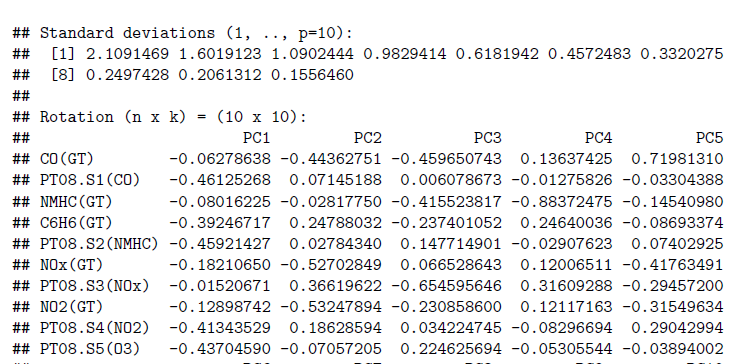
\includegraphics[]{pca5.png}

\smallskip

We will provide a full interpretation of the first two principal components using the principal factor values, with a corresponding plot to illustrate (see below). 

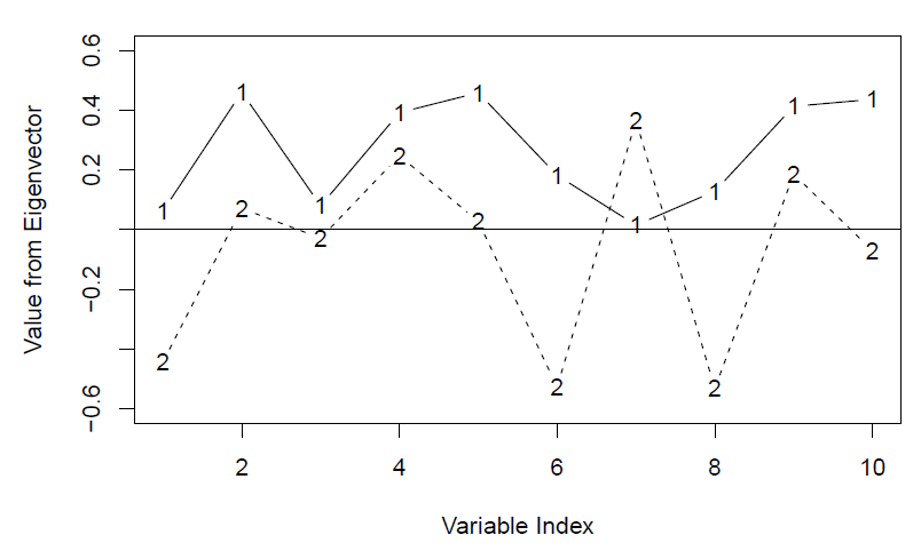
\includegraphics[scale = 0.7]{factorloadings.png}

The first principal component functions as a weighted average of all variables, since all the variable loadings have the same sign. In general, we can think of it as a weighted average representing the overall level of pollution. The primary variables considered by the weighted average are (2) tin oxide sensor response, (4) benzene concentration, (5) titania sensor response, (9) tungston oxide sensor response (NO2 targeted), and (10) indium oxide sensor response. The first principal component is therefore primarily a weighted average of tin oxide, benzene, titania, tungston oxide (NO2 targeted), and indium oxide air pollutants. Observations with higher overall levels of pollution, especially with regards to the above air pollutants, will have higher values for the first principal component.

\smallskip

The second principal component represents the skew between an roughly equal average of variables (1) carbon monoxide concentration, (6) concentration of NOx gases, and (8) nitrogen dioxide concentration against a weighted average of variables (4) benzene concentration, (7) tungsten oxide sensor response (NOx targeted), and (9) tungsten oxide sensor response (NO2 targeted). All other variables have loadings very close to 0 and therefore will not be weighted very strongly in the calculation of PC2 values for individual observations. An observation with high values of carbon monoxide, NOx gases, and nitrogen oxide and low values of benzene and tungsten oxide will have a very negative value for the second principal component.

\smallskip

We can interpret the proportion of variance information contained in the first two principal components using the value $\frac{\lambda_1 + \lambda_2}{\sum^{10}_{j=1}\lambda_j}$, where $\lambda_j$ is the eigenvalue corresponding to the eigenvector of the $j$th principal component. For this selection of the ten air quality variables, the first two principal components alone capture 70.146 percent of the variation.

\smallskip

We will now discuss how to interpret the first two principal components using a small subset of data points from the full data set. 

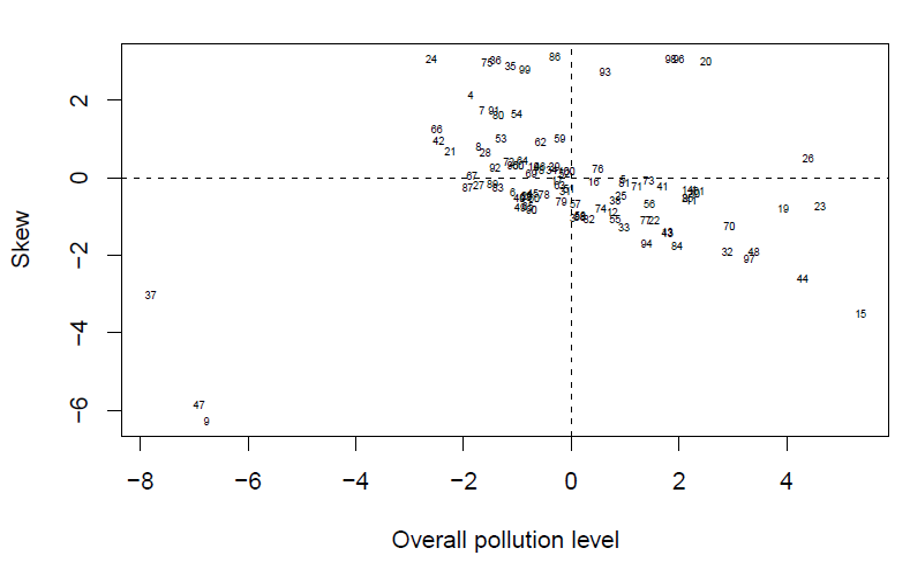
\includegraphics[scale = 0.7]{randomselection.png}

Overall, we see that observations with low overall pollution are generally skewed towards benzene and tungsten oxide; observations with high overall pollution are generally skewed towards carbon monoxide and nitrogen oxide gases. We will interpret a few of the points from the random selection above.

\smallskip

Observation 47 has a strongly negative value for both the first principal component and the second principal component. So at observation 47, overall pollution is low (especially with regards to those pollutants weighted heavily in the first principal component). Additionally, its values of carbon monoxide, NOx gases, and nitrogen oxide will be larger relative to its values of benzene and tungsten oxide.

\smallskip

Observation 24 has a slightly negative value for the first principal component and a strongly positive value for the second principal component. Overall pollution is somewhat low, and the values of benzene and tungsten oxide are relatively high when weighted against the values of carbon monoxide, NOx gases, and nitrogen oxide.

\smallskip

Observation 26 has a high positive value for the first principal component and a value close to zero for the second principal component. Overall pollution is quite high, but there is not much skew when comparing the group of benzene and tungsten oxide against the group of carbon monoxide, NOx gases, and nitrogen oxide.

\smallskip

Observations 15 and 37 have similar values for the second principal component, so they have a similar balance with regards to the skew of the two air pollutant groups considered. However, we can also see that overall pollution is extremely low for observation 37 and extremely high for observation 15. Observation 37 was recorded on August 28, which is a time of year with moderate temperatures. Observation 15 was recorded on November 22, which is colder; this additional heating may be associated with overall higher pollution. Further investigation would be required to see if this idea is supported by the full dataset.

\section{Cluster Analysis in R}
\subsection{Data Scaling and Hierarchical Clustering}

This section of the report mainly focuses on performing \textbf{clustering analysi}s, especially: \par
\begin{itemize}
    \item Group the data and see if components show a related pattern in contribution to environmental pollution, for example, under certain climates, does the density/concentration of chemistry descend/ascend together?
    \item Analyze the seasonality of temperature and pollution density. In other words, in the summer, does $\mathrm{O_3}$ increase while in winter, $\mathrm{CO}$ increase?
\end{itemize}\par

We use hierarchical clustering methods in R Studio. The process can be interpreted as:
\begin{itemize}
    \item Dealing with missing data and scaling:
    \begin{minted}{R}
    data[data == -200] <- NA
    data <- na.omit(data)
    data_numeric <- select(data, -Month)
    data_scaled <- scale(data_numeric)
    \end{minted}
    \item Perform hierarchical clustering using Euclidean Distance:
    \begin{minted}{R}
    d <- dist(data_scaled, method = "euclidean")
    hc <- hclust(d, method = "ward.D2")
    plot(hc)
    k <- 4 
    clusters <- cutree(hc, k = k)
    fviz_cluster(list(data = data_scaled, cluster = clusters))
    \end{minted}
We obtained the clustering results, shown in the figure:
    \begin{figure}[H]
    \centering
    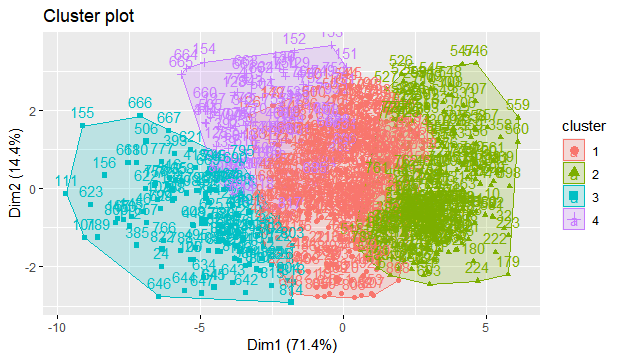
\includegraphics[width=13cm]{Rplot.png}
    \label{fig:unique_label_1}
    \caption{Cluster Plot}
    \end{figure}
\item Then we can check different clusters concerning the original dataset to see the points each cluster contains.
\begin{minted}{R}
    data_with_clusters <- data
    data_with_clusters$Cluster <- clusters
    for (i in 1:k) {
    cat("Cluster", i, ":\n")
    print(data_with_clusters[data_with_clusters$Cluster == i, ])
    cat("\n")}
\end{minted}
 The clustering result can reveal \textbf{which types of air pollutants (such as CO, NOx, PM2.5, etc.) tend to occur under similar environmental conditions.}

\begin{minted}{R}
    Cluster 1 :
# A tibble: 338 × 15
   `CO(GT)` `PT08.S1(CO)` `NMHC(GT)` `C6H6(GT)` `PT08.S2(NMHC)` `NOx(GT)`
      <dbl>         <dbl>      <dbl>      <dbl>           <dbl>     <dbl>
 1      2.6         1360         150      11.9            1046.       166
 2      2           1292.        112       9.40            955.       103
 3      2.2         1402          88       9.00            939.       131
 4      2.2         1376.         80       9.23            948.       172
 5      1.6         1272.         51       6.52            836.       131
 6      2           1333.         64       8.01            900.       174
 7      2.2         1351          87       9.54            960.       129
 8      1.9         1286.         63       7.27            868.       146
 9      2.9         1371         164      11.5            1034.       207
10      2.2         1310          79       8.83            932.       184
# ℹ 328 more rows
# ℹ 9 more variables: `PT08.S3(NOx)` <dbl>, `NO2(GT)` <dbl>, `PT08.S4(NO2)` <dbl>,
#   `PT08.S5(O3)` <dbl>, T <dbl>, RH <dbl>, AH <dbl>, Month <chr>, Cluster <int>
# ℹ Use `print(n = ...)` to see more rows

Cluster 2 :
# A tibble: 276 × 15
   `CO(GT)` `PT08.S1(CO)` `NMHC(GT)` `C6H6(GT)` `PT08.S2(NMHC)` `NOx(GT)`
      <dbl>         <dbl>      <dbl>      <dbl>           <dbl>     <dbl>
 1      1.2         1197          38       4.74            750.        89
 2      1.2         1185          31       3.62            690.        62
 3      1           1136.         31       3.33            672         62
 4      0.9         1094          24       2.34            608.        45
 5      0.7         1066           8       1.13            512         16
 6      0.7         1052.         16       1.60            553.        34
 7      1.1         1144          29       3.24            667         98
 8      1.7         1233.         77       6.34            827.       112
 9      1.5         1179.         43       4.97            762         95
10      1.6         1236          61       5.22            774.       104
# ℹ 266 more rows
# ℹ 9 more variables: `PT08.S3(NOx)` <dbl>, `NO2(GT)` <dbl>, `PT08.S4(NO2)` <dbl>,
#   `PT08.S5(O3)` <dbl>, T <dbl>, RH <dbl>, AH <dbl>, Month <chr>, Cluster <int>
# ℹ Use `print(n = ...)` to see more rows

Cluster 3 :
# A tibble: 120 × 15
   `CO(GT)` `PT08.S1(CO)` `NMHC(GT)` `C6H6(GT)` `PT08.S2(NMHC)` `NOx(GT)`
      <dbl>         <dbl>      <dbl>      <dbl>           <dbl>     <dbl>
 1      4.8         1581.        307       20.8           1318.       281
 2      6.9         1776.        461       27.4           1488.       383
 3      6.1         1640         401       24.0           1404        351
 4      6.6         1843         488       32.6           1610.       340
 5      4.4         1598.        333       20.1           1299        274
 6      5.4         1677.        367       21.8           1346        300
 7      5.9         1898         341       23.1           1381.       325
 8      5.5         1797.        336       25.9           1451        360
 9      8.1         1961.        618       36.7           1701        478
10      5.8         1770.        438       26.6           1470        394
# ℹ 110 more rows
# ℹ 9 more variables: `PT08.S3(NOx)` <dbl>, `NO2(GT)` <dbl>, `PT08.S4(NO2)` <dbl>,
#   `PT08.S5(O3)` <dbl>, T <dbl>, RH <dbl>, AH <dbl>, Month <chr>, Cluster <int>
# ℹ Use `print(n = ...)` to see more rows

Cluster 4 :
# A tibble: 93 × 15
   `CO(GT)` `PT08.S1(CO)` `NMHC(GT)` `C6H6(GT)` `PT08.S2(NMHC)` `NOx(GT)`
      <dbl>         <dbl>      <dbl>      <dbl>           <dbl>     <dbl>
 1      3.9         1510.        233       19.3           1276.       206
 2      3.7         1525.        242       18.2           1246        202
 3      4.1         1542.        283       16.1           1184.       296
 4      3.6         1451.        210       14.0           1117.       239
 5      3.2         1473.        191       15.5           1163.       227
 6      4.2         1609         258       19.6           1286.       277
 7      4.2         1611.        284       19.2           1274        279
 8      4.2         1620.        269       18.3           1247.       283
 9      4.6         1808.        262       20.6           1312.       261
10      4.2         1564.        334       20.1           1300.       319
# ℹ 83 more rows
# ℹ 9 more variables: `PT08.S3(NOx)` <dbl>, `NO2(GT)` <dbl>, `PT08.S4(NO2)` <dbl>,
#   `PT08.S5(O3)` <dbl>, T <dbl>, RH <dbl>, AH <dbl>, Month <chr>, Cluster <int>
# ℹ Use `print(n = ...)` to see more rows
\end{minted}
\end{itemize}
\subsection{Clustering under Temperature and Humidity}
We can also investigate the correlation between nitrogen oxides (NOx) and nitrogen dioxide (NO2) under different environmental conditions since we performed clustering analysis.
    \begin{minted}{R}
    selected_vars <- c("T", "RH", "CO(GT)", "NOx(GT)", "NO2(GT)")
    ggpairs(data_with_clusters[, selected_vars], aes(colour = as.factor(Cluster)))

    for (i in selected_vars) {
    for (j in selected_vars) {
    if (i != j) {
    p <- ggplot(data_with_clusters, aes(x = !!sym(i), y = !!sym(j), colour = Cluster)) +
    geom_point() +
    theme_minimal() +
    ggtitle(paste("Scatter plot of", i, "vs", j))
    print(p)}}}
    
    \end{minted}

\begin{figure}[H]
    \centering
    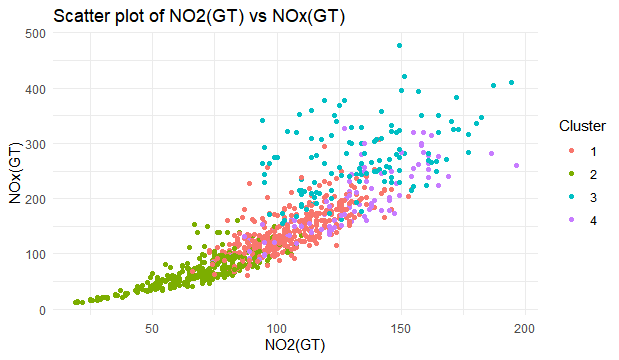
\includegraphics[width=13cm]{Rplot02.png}
    \label{fig:unique_label_1}
    \caption{Correlation between NO2 and Nox}
    \end{figure}
    For example, the Green Cluster (0 to 50-100) may represent an environmental condition where the concentrations of NOx(GT) and NO2(GT) are relatively low and exhibit a strong positive correlation. This suggests that under this environmental condition, NOx and NO2 concentrations typically increase or decrease together.\par
    We also investigated the correlation between temperature and $NO_x$:
    \begin{minted}{R}
    selected_vars <- c("T", "NOx(GT)")
    ggpairs(data_with_clusters[, selected_vars], aes(colour = as.factor(Cluster)))
    p <- ggplot(data_with_clusters, aes(x = T, y = `NOx(GT)`, colour = Cluster)) +
    geom_point() +
    theme_minimal() +
    ggtitle("Scatter plot of T vs NOx")
    print(p)

    \end{minted}
    \begin{figure}[H]
    \centering
    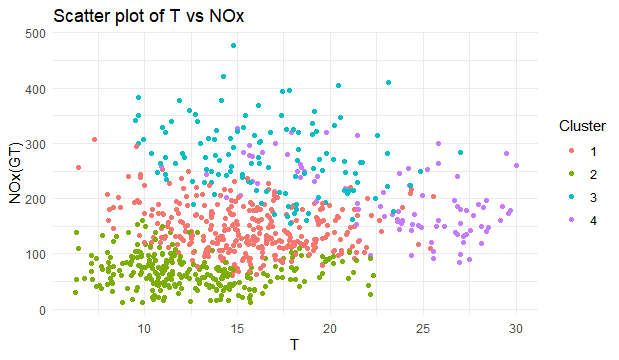
\includegraphics[width=13cm]{Rplot03.png}
    \label{fig:unique_label_1}
    \caption{Correlation between temperature and NOx}
    \end{figure}

\section{References}

Vito, Saverio. (2016). Air Quality. UCI Machine Learning Repository.
https://doi.org/10.24432/C59K5F.

\end{document}
